\section{TUNGGAL (Solo Performance) Category}
\label{sec:tunggal_category}


\begin{legal}
\item Competition Equipment:
    \begin{legal}
    \item \strong{Attire:}\\

    A standard Pencak Silat attire (Figure~\ref{fig:tunggal_ganda_attire} of any color and plain (The top and bottom pieces may be of the same or different color). A headband (a veil not covering face, is not consider as a headband) and ‘kain samping’ of plain color or patterned. The color choice and combination are entirely at the discretion of the Contestant. It is allowed to have the badge of the contestant’s main association on the left chest and PERSILAT badge on the right chest. The national flag on the left arm and the name of the country at the upper back of the attire.

    
    \item \strong{Weapons:}\\
    For Senior, golok or parang (Figure~\ref{fig:golok}) is made of metal or wood, non-sharp pointed with length 
    between 30 cm up to 40cm and width of between 2.5 cm to 4 cm.  `Toya' (staff) (Figure~\ref{fig:toya}), 
    is made of rattan with the length of between 150-180 cm and diameter of between 2.5-3.5 cm.

    \begin{figure}[t!]
    \centering
    \subfigure[Tunggal / Ganda Attire]{\label{fig:tunggal_ganda_attire}
        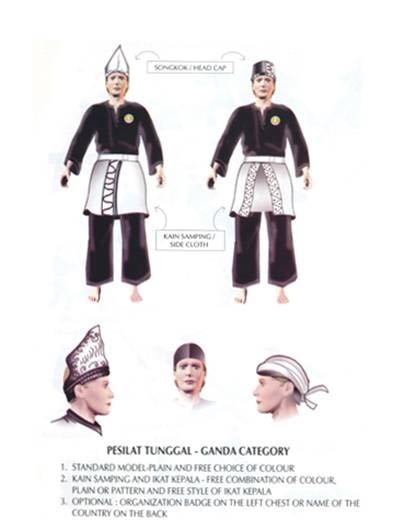
\includegraphics[height=3.0in]{images/tunggal_ganda_attire}
    }
    ~
    \subfigure[Golok / Machete]{\label{fig:golok}
        
\includegraphics[height=2.5in]{images/golok}
    }
    ~
    \subfigure[Toya / Staff ]{\label{fig:toya}
        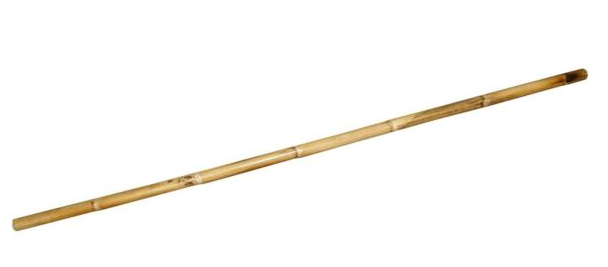
\includegraphics[width=5.0in]{images/toya}
    }
    \caption{Tunggal Weapons}
    \end{figure}

    \end{legal}

\item Competition Stages

    \begin{legal}
    \item When a competition is participated by more than 7 (seven) contestants, a pool system will be implemented.
    \item The three (3) contestants with the highest scores from each pool will compete again in the next round. 
    Unless the following round is the final. The participants of the final round will be the best 3 (three) – in 
    terms of gaining scores – from the previous competition pool stages.
    \item The number of pools is decided in a meeting attended by International Technical Delegates, 
    Competition Chairperson and Council of Jury. The decision will be announced to the participants at the 
    Technical Meeting.
    \item The pool division for contestants is determined by drawing of lots during the Technical Meeting. 
    Voting method, i.e either manually or digitally will be decided through voting at the Technical Meeting.
    \item \underline{Each category should be have a minimum of 2 (two) participants.} When there are only two participants
    competition goes directly to the final round.
    \end{legal}



\item Duration of Competition\\
The performance duration is 3 (three) minutes.

    \begin{figure}[ht!]
    \centering
    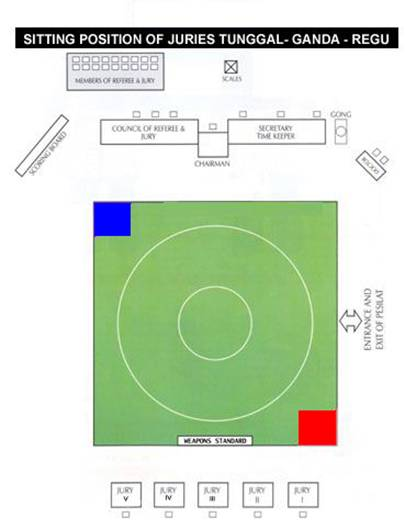
\includegraphics[height=4.0in]{images/performance_arena}
    \caption{Performance Arena}
    \label{fig:performance_arena}
    \end{figure}



\item Competition Procedure
    \begin{legal}
    \item The beginning of competition:
        \begin{enumerate}[label=\alph*.]
        \item Juries reporting for duty to the Competition Chairperson from the right side of the Competition Chairperson
        \item Show respect and readiness to perform duty
        \item Taking the allocated seats
        \end{enumerate}

    \item The weapons that were certified by the Competition Chairperson will be placed at the weapon quarantine station as prepared by the organizing committee.\\

Pesilat/coach will be allowed to collect the weapons just before he/she enter the arena (immediately after his/her name was announced).

    \item Pesilat
        \begin{enumerate}[label=\alph*.]
        \item Entering the arena from the left side of the Competition Chairperson
        \item Walk towards the centre of arena
        \item Pesilat is to place the weapon on the weapon stand (no assistance from coach)
        \item Show respect to the Competition Chairperson and turn back to show respect to the Jury
        \end{enumerate}

    \item Competition Chairperson will signal the Jury, time keeper and other competition officials to alert them 
        that duty is about to begin

    \item The showcase
        \begin{enumerate}[label=\alph*.]
        \item Showcase the Opening PERSILAT greeting
        \item The gong will be stricken to mark the beginning of performance time. Contestant to begin the showcase
        \item Bare hand movement
        \item With the Long knife / Golok
        \item With the long stick / Toya (staff)
        \item The gong will be stricken to mark the end of performing time
        \end{enumerate}
    
    \item At the end of the performance
        \begin{enumerate}[label=\alph*.]
        \item Contestant to show respect to the Jury and Competition Chairperson from the center of the arena
        \item To leave the arena by the left side of the Competition Chairperson
        \end{enumerate}

    \item Time Keeping
        \begin{enumerate}[label=\alph*.]
        \item The Competition Chairperson will make sure / take charge of the showcase time.
        \item The time keeper will keep track of the 3 minutes showcase.
        \item Competition Chairperson will announce the actual showcase time. (If digital scoring is used, 
            the time tracking will be as displayed on the screen)
        \end{enumerate}

    \end{legal}

\item Competition Rules

    \begin{legal}
    \item Rules of the game

        \begin{legal}
        \item Contestant showcases the Jurus Tunggal Baku (Solo Compulsory Movement) in three (3) minutes, 
            begin with bare hand followed with weapon movement follow with long knife (golok) followed by the 
            long stick (toya). \\

            A tolerance period of +/-10 seconds is allowed for Pre-teen and Pre-Junior categories while +/-5 
            seconds for the Junior, Senior and Masters categories.\\

            Should the tolerance period go beyond the limit, penalty will be imposed accordingly.
        
        \item Jurus Tunggal Baku is showcased according to the sequential movement, 
            such as the fixed movement sequence, precise techniques with and without weapons, rhythmic movement, 
            firmness and expression.

        \item \label{pt:failed_to_continue} If the contestant failed to continue his/her performance for whatever reason, the  
            Competition Chairperson will declare he/she as being disqualified.

        \item Uttering of voice is allowed.
        \end{legal}

    \item Penalties
        \begin{legal}
        \item \label{pt:tunggal_deductions} Deduction of points will be imposed as such:
            \begin{enumerate}[label=\alph*.]

            \item Mistake in movement sequence and techniques
                \begin{enumerate}[label*=\arabic*.]
                \item Deduction of one (1) point each time
                    \begin{enumerate}[label=\roman*.]
                    \item mistake in movement sequence details
                    \item mistake in movement techniques
                    \item any missing movement (not done)
                    \item should a Pesilat lose grip of the weapon, as long as it does not touches the ground, 
                        a total of 1 point penalty for each wrong and/or additional movement incurred. 
                    \end{enumerate}
                \end{enumerate}

            \item Time factor
                \begin{enumerate}[label*=\arabic*.]
                \item \label{pt:tunggal_deduction_beyond_time} Beyond tolerance period \\
                    Ten (10) to fifteen (15) seconds – deduction of 10 points for Pre-teen and Pre-Junior 
                    categories and five (5) to ten (10) seconds for Junior, Senior and masters categories.\\

                    Should showcase go beyond these tolerance period the showcase will be stopped and 
                    declared disqualified.
                \end{enumerate}


            \item Other factors
                \begin{enumerate}[label*=\arabic*.]
                \item Exceed the arena limit (10m x 10m) – Deduction of 5 points
                \item Drop of weapon – Deduction of 5 points
                \item Attires is not according to prescription – Deduction of 5 points 
                (eg. Extra accessories, head gear or samping fall or)
                \item \label{pt:tunggal_loose_weapon} Weapon came out loose from the handle or breaking of the long stick. 
                Showcase will be stopped and declared disqualified.
                \end{enumerate}
            \end{enumerate}

        \end{legal}

        \item Other Decisions
            \begin{legal}
            \item The Referee Jury Council has the right to request for amendments of the penalties 
            (impose penalty or withdraw penalty) following 3 or more Jury views and decision. Penalty imposed will be denied if it is only be given by 2 or 1 Jury.
            \item When competition is unable to continue due to:
                \begin{enumerate}[label*=\roman*.]
                \item Juries failed to function (fall sick / injured / unconscious)
                \item Non-Technical factors (Electrical breakdown / disturbance / etc)
                \item External factors (something that is beyond human control, natural disaster etc)

                \end{enumerate}

                \begin{enumerate}[label*=\alph*.]
                    \item Competition chairperson will stop the competition with following guidelines:

                    \begin{enumerate}[label*=\arabic*.]
                    \item Contestant involve (unless the last contestant) will be allowed to showcase the performance again right from the beginning (at whichever round he is contesting) with the same Juries, right after the last contestant completing his/her showcase.
                    \item If it is during the last contestant showcase, contestant will be allowed to re-showcase his performance from the beginning, at the latest 10 minutes after the technical problem is solved.
                    \item The Jury that could not carry out their duty is to be replaced.
                    \end{enumerate}
                \end{enumerate}

            \item \label{pt:tunggal_accident} Competition could not proceed due to any accident caused by the contestant (collision with 
                Juries / Jury was hurt due to weapon flung to them, etc) Contestant will be disqualified. 
                Competition Chairperson will replace the injured Jury (after consultation with Technical Delegate) 
                and competition will resume with the next contestant.
            \end{legal}

            \item Walk-over \\
                Participation will be declared as Walk-over should the contestant fail to report to 
                Competition’s Secretary after being call for the 3rd time.\\
                The interval between the call outs will be at thirty (30) seconds each.

            \item Disqualification \\
                \begin{enumerate}[label*=\arabic*.]
                \item Points given to contestant will be withdrawn should it be realized 
                    (at the end of the showcase) that the contestant failed to showcase the whole package or 
                    had perform the package sequence not in proper order.
                \item Putting on totally non-proper attire (not as stipulated) or using a wrong weapon 
                    (eg. Tombak instead of toya)
                \item Pesilat is unable to continue the showcase due to his own fault.
                \item Matters that are stated at point \ref{pt:failed_to_continue}, \ref{pt:tunggal_deductions} (\ref{pt:tunggal_deduction_beyond_time}), \ref{pt:tunggal_deductions} \ref{pt:tunggal_loose_weapon}, and \ref{pt:tunggal_accident}.
                \item Pesilat is unable to show the letter of medical checkup before starting the first match (regardless of category) of the competition.
                \end{enumerate}

    \end{legal}

\item Scoring
    \begin{legal}
    \item Scoring consists of:
        \begin{legal}
        \item Accuracy score includes the following elements:
            \begin{enumerate}[label*=\alph*.]
            \item The accuracy of movement in each Jurus
            \item The accuracy of movement sequence
            \item The accuracy of jurus sequence

            \end{enumerate}

        The score is obtained from the total number of movements in Jurus Tunggal (100 movements) 
        deducted by the penalty points.

        \item Firmness scores include the following elements:
            \begin{enumerate}[label*=\alph*.]
            \item The firmness of movements
            \item The firmness of movement rhythm
            \item The firmness of movement soulfulness
            \item The firmness of power and stamina
            \end{enumerate}

        Score ranges from 50 to 60 points which is the accumulated score of the four firmness elements.
        \end{legal}

    \end{legal}

\item Decision and announcement of the winner
    \begin{legal}
    \item  \label{pt:tunggal_hi_score} The winner is the contestant who gains the highest score for his/her performance from 3 (three) out of 5 (five) jurors with elimination of the highest and the lowest score.
    \item If the scores are equal, the winner will be determined accordingly:
            \begin{enumerate}[label*=\roman*.]
            \item The contestant who gains the total highest Technique points from the 3 (three) jurors as decided in para \ref{pt:tunggal_hi_score}.
            \item The contestant who gains the highest points in firmness, soulfulness and stamina from 3 (three) jurors as decided in para \ref{pt:tunggal_hi_score}.
            \item The contestant whose duration of performance is the closest to precise time of 3 (three) minutes.
            \item The winner is the contestant who gains the least penalty points.
            \item If the result remains the same, the Competition Chairperson will do a coin toss on to the mat witnessed by Technical Delegate, Council of Juror and Team Managers of respective contestant.
            \end{enumerate}

    \item The score of each contestant is announced after the Jury has finished their task in giving score to all contestant of every Jurus Tunggal (Solo Performance) category. Total obtained scores will be shown in scoreboard while announced by Competition Chairperson except when using digital scoreboard where the scores from each Jury and total scores are displayed in the screen instantly.
    \end{legal}

\end{legal}
